\documentclass[a4paper]{report}
\usepackage{sol_manual}
\author{Pingbang Hu}
\title{High-Dimensional Probability\\Solution Manual}

\thispagestyle{empty}
\addbibresource{ref.bib}
\addbibresource{~/Research/Zotero/My Library.bib}

\begin{document}

\maketitle

\begin{abstract}
	This is the solution I write when organizing the reading group on \href{https://www.math.uci.edu/~rvershyn/}{Roman Vershynin}'s \emph{High Dimensional Probability}~\cite{vershyninHighDimensionalProbability2024}. While we aim to solve all the exercises, occasionally we omit some due to either
	\begin{enumerate*}[label=\arabic*.)]
		\item simplicity;
		\item difficulty; or
		\item skipped section.
	\end{enumerate*}
	Additionally, it may contain factual and/or typographic errors.

	\vfill
	\begin{center}
		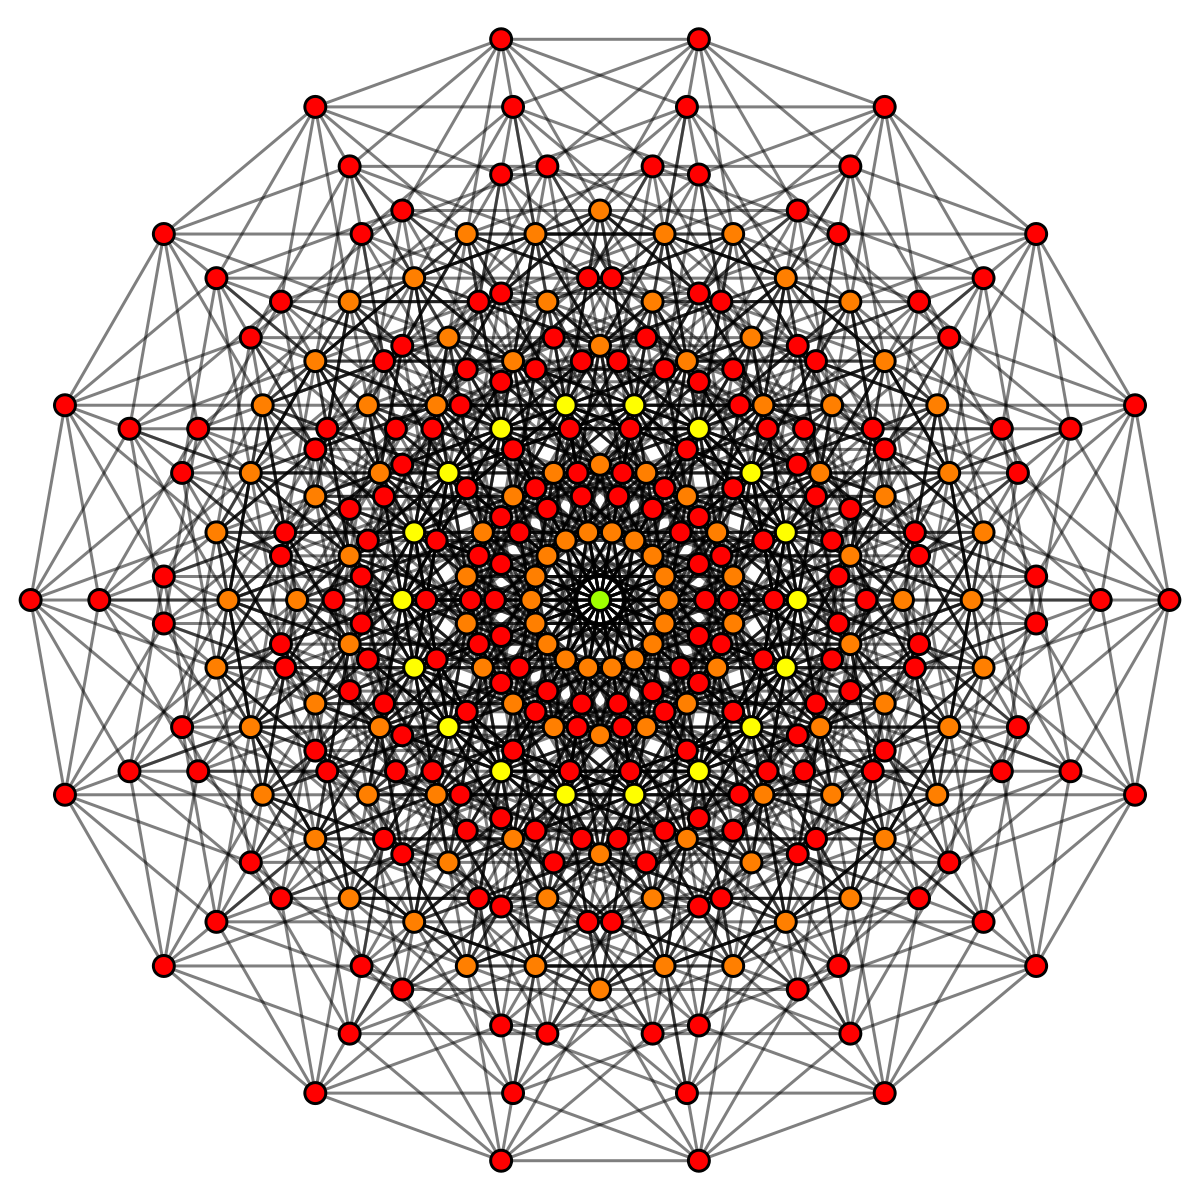
\includegraphics[width=\linewidth]{Figures/cover.png}
	\end{center}
	\vfill
	The reading group started from Spring 2024, and the date on the cover page is the last updated time.
\end{abstract}

\tableofcontents

\wk{1}{16}

% \newpage
% %─────Appendix────────────────────────────────────────────────────────────────────────────────────────────────────────────────────────────────────────
% \appendix
% \appendixpage{}

% \input{appendix.tex}

\newpage
%─────Reference──────────────────────────────────────────────────────────────────────────────────────────────────────────────────────────────────────
\printbibliography{}

\end{document}